\documentclass[10pt,aspectratio=169,dvipsnames]{beamer}
\usepackage{pgfpages}
\graphicspath{{./figures/}{./logos/}}
\usetheme[progressbar=frametitle, sectionpage=none]{metropolis}
\usepackage{appendixnumberbeamer}
\usepackage{siunitx}
\usepackage{framed}
\usepackage{color}
\usepackage{hyperref}
\usepackage{minted}
\usepackage{txfonts}
% Add functionality to includegraphics for adding labels.
% From: https://tex.stackexchange.com/questions/454660/adding-a-label-on-top-of-figure
% Options:
% pos = nw | n | ne | e | se | s | sw | w
% labelbox = true | false
% fontsize = <fontsize command>
% Examples:
% \xincludegraphics[scale=0.3,label=a)]{example-image-a}
% \xincludegraphics[scale=0.3,label=b)]{example-image-b}
% \xincludegraphics[scale=0.2,angle=90,label=c),pos=sw,labelbox,fontsize=\Large]{example-image-c}
% \xincludegraphics[scale=0.2,angle=90,label=c),pos=w,labelbox,fontsize=\tiny]{example-image-c}
% \setlabel{pos=ne,fontsize=\scriptsize,labelbox}
% \xincludegraphics[scale=0.2,angle=90,label=x)]{example-image-c}
% \xincludegraphics[scale=0.2,angle=90,label=y),labelbox=false]{example-image-c}
%
% Include using % Add functionality to includegraphics for adding labels.
% From: https://tex.stackexchange.com/questions/454660/adding-a-label-on-top-of-figure
% Options:
% pos = nw | n | ne | e | se | s | sw | w
% labelbox = true | false
% fontsize = <fontsize command>
% Examples:
% \xincludegraphics[scale=0.3,label=a)]{example-image-a}
% \xincludegraphics[scale=0.3,label=b)]{example-image-b}
% \xincludegraphics[scale=0.2,angle=90,label=c),pos=sw,labelbox,fontsize=\Large]{example-image-c}
% \xincludegraphics[scale=0.2,angle=90,label=c),pos=w,labelbox,fontsize=\tiny]{example-image-c}
% \setlabel{pos=ne,fontsize=\scriptsize,labelbox}
% \xincludegraphics[scale=0.2,angle=90,label=x)]{example-image-c}
% \xincludegraphics[scale=0.2,angle=90,label=y),labelbox=false]{example-image-c}
%
% Include using % Add functionality to includegraphics for adding labels.
% From: https://tex.stackexchange.com/questions/454660/adding-a-label-on-top-of-figure
% Options:
% pos = nw | n | ne | e | se | s | sw | w
% labelbox = true | false
% fontsize = <fontsize command>
% Examples:
% \xincludegraphics[scale=0.3,label=a)]{example-image-a}
% \xincludegraphics[scale=0.3,label=b)]{example-image-b}
% \xincludegraphics[scale=0.2,angle=90,label=c),pos=sw,labelbox,fontsize=\Large]{example-image-c}
% \xincludegraphics[scale=0.2,angle=90,label=c),pos=w,labelbox,fontsize=\tiny]{example-image-c}
% \setlabel{pos=ne,fontsize=\scriptsize,labelbox}
% \xincludegraphics[scale=0.2,angle=90,label=x)]{example-image-c}
% \xincludegraphics[scale=0.2,angle=90,label=y),labelbox=false]{example-image-c}
%
% Include using \input{xincludegraphics.tex} before \begin{document}
% \xincludegraphics[width=0.9\textwidth, label=a),labelbox,fontsize=\small]{.image.png}
\usepackage{graphicx}
\usepackage{xcolor}
\usepackage{xparse,xcoffins}

\ExplSyntaxOn
\NewCoffin\imagecoffin
\NewCoffin\labelcoffin

\keys_define:nn { miguel/label }
 {
  label   .tl_set:N = \l_miguel_label_tl,
  labelbox .bool_set:N = \l_miguel_label_box_bool,
  labelbox .default:n = true,
  fontsize .tl_set:N = \l_miguel_label_size_tl,
  fontsize .initial:n = \footnotesize,
  pos .choice:,
  pos/nw .code:n = \tl_set:Nn \l_miguel_label_pos_tl { left,up },
  pos/ne .code:n = \tl_set:Nn \l_miguel_label_pos_tl { right,up },
  pos/sw .code:n = \tl_set:Nn \l_miguel_label_pos_tl { left,down },
  pos/se .code:n = \tl_set:Nn \l_miguel_label_pos_tl { right,down },
  pos/n .code:n = \tl_set:Nn \l_miguel_label_pos_tl { hc,up },
  pos/w .code:n = \tl_set:Nn \l_miguel_label_pos_tl { left,vc },
  pos/s .code:n = \tl_set:Nn \l_miguel_label_pos_tl { hc,down },
  pos/e .code:n = \tl_set:Nn \l_miguel_label_pos_tl { right,vc },
  pos .initial:n = nw,
  unknown .code:n   = \clist_put_right:Nx \l_miguel_label_clist
                       { \l_keys_key_tl = \exp_not:n { #1 } }
 }
\clist_new:N \l_miguel_label_clist
\box_new:N \l_miguel_label_box
\box_new:N \l_miguel_label_image_box

\NewDocumentCommand{\xincludegraphics}{O{}m}
 {
  \group_begin:
  \tl_clear:N \l_miguel_label_tl
  \clist_clear:N \l_miguel_label_clist
  \keys_set:nn { miguel/label } { #1 }
  \tl_if_empty:NTF \l_miguel_label_tl
   {
    \miguel_includegraphics:Vn \l_miguel_label_clist { #2 }
   }
   {
    \SetHorizontalCoffin\imagecoffin
     {
      \miguel_includegraphics:Vn \l_miguel_label_clist { #2 }
     }
    \SetHorizontalCoffin\labelcoffin
     {
      \raisebox{\depth}
       {
        \bool_if:NTF \l_miguel_label_box_bool
         { \fcolorbox{white}{white}{\l_miguel_label_size_tl\l_miguel_label_tl} }
         { \l_miguel_label_size_tl\l_miguel_label_tl }
       }
     }
    \SetVerticalPole\imagecoffin{left}{3pt+\CoffinWidth\labelcoffin/2}
    \SetVerticalPole\imagecoffin{right}{\Width-3pt-\CoffinWidth\labelcoffin/2}
    \SetHorizontalPole\imagecoffin{up}{\Height-3pt-\CoffinHeight\labelcoffin/2}
    \SetHorizontalPole\imagecoffin{down}{3pt+\CoffinHeight\labelcoffin/2}
    \use:x{\JoinCoffins\imagecoffin[\l_miguel_label_pos_tl]\labelcoffin[vc,hc]} 
    \TypesetCoffin\imagecoffin
   }
   \group_end:
 }
\NewDocumentCommand{\setlabel}{m}
 {
  \keys_set:nn { miguel/label } { #1 }
 }

\cs_new_protected:Nn \miguel_includegraphics:nn
 {
  \includegraphics[#1]{#2}
 }
\cs_generate_variant:Nn \miguel_includegraphics:nn { V }

\ExplSyntaxOff
 before \begin{document}
% \xincludegraphics[width=0.9\textwidth, label=a),labelbox,fontsize=\small]{.image.png}
\usepackage{graphicx}
\usepackage{xcolor}
\usepackage{xparse,xcoffins}

\ExplSyntaxOn
\NewCoffin\imagecoffin
\NewCoffin\labelcoffin

\keys_define:nn { miguel/label }
 {
  label   .tl_set:N = \l_miguel_label_tl,
  labelbox .bool_set:N = \l_miguel_label_box_bool,
  labelbox .default:n = true,
  fontsize .tl_set:N = \l_miguel_label_size_tl,
  fontsize .initial:n = \footnotesize,
  pos .choice:,
  pos/nw .code:n = \tl_set:Nn \l_miguel_label_pos_tl { left,up },
  pos/ne .code:n = \tl_set:Nn \l_miguel_label_pos_tl { right,up },
  pos/sw .code:n = \tl_set:Nn \l_miguel_label_pos_tl { left,down },
  pos/se .code:n = \tl_set:Nn \l_miguel_label_pos_tl { right,down },
  pos/n .code:n = \tl_set:Nn \l_miguel_label_pos_tl { hc,up },
  pos/w .code:n = \tl_set:Nn \l_miguel_label_pos_tl { left,vc },
  pos/s .code:n = \tl_set:Nn \l_miguel_label_pos_tl { hc,down },
  pos/e .code:n = \tl_set:Nn \l_miguel_label_pos_tl { right,vc },
  pos .initial:n = nw,
  unknown .code:n   = \clist_put_right:Nx \l_miguel_label_clist
                       { \l_keys_key_tl = \exp_not:n { #1 } }
 }
\clist_new:N \l_miguel_label_clist
\box_new:N \l_miguel_label_box
\box_new:N \l_miguel_label_image_box

\NewDocumentCommand{\xincludegraphics}{O{}m}
 {
  \group_begin:
  \tl_clear:N \l_miguel_label_tl
  \clist_clear:N \l_miguel_label_clist
  \keys_set:nn { miguel/label } { #1 }
  \tl_if_empty:NTF \l_miguel_label_tl
   {
    \miguel_includegraphics:Vn \l_miguel_label_clist { #2 }
   }
   {
    \SetHorizontalCoffin\imagecoffin
     {
      \miguel_includegraphics:Vn \l_miguel_label_clist { #2 }
     }
    \SetHorizontalCoffin\labelcoffin
     {
      \raisebox{\depth}
       {
        \bool_if:NTF \l_miguel_label_box_bool
         { \fcolorbox{white}{white}{\l_miguel_label_size_tl\l_miguel_label_tl} }
         { \l_miguel_label_size_tl\l_miguel_label_tl }
       }
     }
    \SetVerticalPole\imagecoffin{left}{3pt+\CoffinWidth\labelcoffin/2}
    \SetVerticalPole\imagecoffin{right}{\Width-3pt-\CoffinWidth\labelcoffin/2}
    \SetHorizontalPole\imagecoffin{up}{\Height-3pt-\CoffinHeight\labelcoffin/2}
    \SetHorizontalPole\imagecoffin{down}{3pt+\CoffinHeight\labelcoffin/2}
    \use:x{\JoinCoffins\imagecoffin[\l_miguel_label_pos_tl]\labelcoffin[vc,hc]} 
    \TypesetCoffin\imagecoffin
   }
   \group_end:
 }
\NewDocumentCommand{\setlabel}{m}
 {
  \keys_set:nn { miguel/label } { #1 }
 }

\cs_new_protected:Nn \miguel_includegraphics:nn
 {
  \includegraphics[#1]{#2}
 }
\cs_generate_variant:Nn \miguel_includegraphics:nn { V }

\ExplSyntaxOff
 before \begin{document}
% \xincludegraphics[width=0.9\textwidth, label=a),labelbox,fontsize=\small]{.image.png}
\usepackage{graphicx}
\usepackage{xcolor}
\usepackage{xparse,xcoffins}

\ExplSyntaxOn
\NewCoffin\imagecoffin
\NewCoffin\labelcoffin

\keys_define:nn { miguel/label }
 {
  label   .tl_set:N = \l_miguel_label_tl,
  labelbox .bool_set:N = \l_miguel_label_box_bool,
  labelbox .default:n = true,
  fontsize .tl_set:N = \l_miguel_label_size_tl,
  fontsize .initial:n = \footnotesize,
  pos .choice:,
  pos/nw .code:n = \tl_set:Nn \l_miguel_label_pos_tl { left,up },
  pos/ne .code:n = \tl_set:Nn \l_miguel_label_pos_tl { right,up },
  pos/sw .code:n = \tl_set:Nn \l_miguel_label_pos_tl { left,down },
  pos/se .code:n = \tl_set:Nn \l_miguel_label_pos_tl { right,down },
  pos/n .code:n = \tl_set:Nn \l_miguel_label_pos_tl { hc,up },
  pos/w .code:n = \tl_set:Nn \l_miguel_label_pos_tl { left,vc },
  pos/s .code:n = \tl_set:Nn \l_miguel_label_pos_tl { hc,down },
  pos/e .code:n = \tl_set:Nn \l_miguel_label_pos_tl { right,vc },
  pos .initial:n = nw,
  unknown .code:n   = \clist_put_right:Nx \l_miguel_label_clist
                       { \l_keys_key_tl = \exp_not:n { #1 } }
 }
\clist_new:N \l_miguel_label_clist
\box_new:N \l_miguel_label_box
\box_new:N \l_miguel_label_image_box

\NewDocumentCommand{\xincludegraphics}{O{}m}
 {
  \group_begin:
  \tl_clear:N \l_miguel_label_tl
  \clist_clear:N \l_miguel_label_clist
  \keys_set:nn { miguel/label } { #1 }
  \tl_if_empty:NTF \l_miguel_label_tl
   {
    \miguel_includegraphics:Vn \l_miguel_label_clist { #2 }
   }
   {
    \SetHorizontalCoffin\imagecoffin
     {
      \miguel_includegraphics:Vn \l_miguel_label_clist { #2 }
     }
    \SetHorizontalCoffin\labelcoffin
     {
      \raisebox{\depth}
       {
        \bool_if:NTF \l_miguel_label_box_bool
         { \fcolorbox{white}{white}{\l_miguel_label_size_tl\l_miguel_label_tl} }
         { \l_miguel_label_size_tl\l_miguel_label_tl }
       }
     }
    \SetVerticalPole\imagecoffin{left}{3pt+\CoffinWidth\labelcoffin/2}
    \SetVerticalPole\imagecoffin{right}{\Width-3pt-\CoffinWidth\labelcoffin/2}
    \SetHorizontalPole\imagecoffin{up}{\Height-3pt-\CoffinHeight\labelcoffin/2}
    \SetHorizontalPole\imagecoffin{down}{3pt+\CoffinHeight\labelcoffin/2}
    \use:x{\JoinCoffins\imagecoffin[\l_miguel_label_pos_tl]\labelcoffin[vc,hc]} 
    \TypesetCoffin\imagecoffin
   }
   \group_end:
 }
\NewDocumentCommand{\setlabel}{m}
 {
  \keys_set:nn { miguel/label } { #1 }
 }

\cs_new_protected:Nn \miguel_includegraphics:nn
 {
  \includegraphics[#1]{#2}
 }
\cs_generate_variant:Nn \miguel_includegraphics:nn { V }

\ExplSyntaxOff

\hypersetup{
colorlinks, urlcolor=blue, linkcolor={blue!10!black},
citecolor={blue!50!black}
}
\usepackage[natbib=true,style=authoryear,backend=bibtex,useprefix=true]{biblatex}
\addbibresource{references.bib}
%
% metropolis theme: https://github.com/matze/mtheme
%
\mode<presentation>
{
  \usetheme{metropolis}      % or try Darmstadt, Madrid, Warsaw, ...
  %\usecolortheme{default} % or try albatross, beaver, crane, ...
  %\usefonttheme{default}  % or try serif, structurebold, ...
  \setbeamertemplate{navigation symbols}{}
  \setbeamertemplate{caption}[numbered]
} 
\definecolor{kitwaregray}{HTML}{686868}
\definecolor{kitwarelightgray}{HTML}{EEEEEE}
\definecolor{kitwareblue}{HTML}{005F9E}
\definecolor{kitwaregreen}{HTML}{009D49}
\definecolor{kitwarewhite}{HTML}{FFFFFF}
\definecolor{kitwareblack}{HTML}{000000}
\definecolor{shadecolor}{HTML}{EEEEEE}

\setbeamercolor{progress bar}{fg=kitwaregreen}
% Theme colors are derived from these two elements
%\setbeamercolor{alerted text}{fg=}
\setbeamercolor{frametitle}{bg=kitwareblue}
\setbeamercolor{footline}{bg=kitwaregreen}
\setbeamerfont{frame numbering}{size=\small}
\setbeamertemplate{footline}{%
  \begin{beamercolorbox}[wd=\textwidth, sep=1ex]{footline}%
    %\usebeamerfont{page number in head/foot}%
    \usebeamertemplate*{frame footer}
    \hfill%
    \usebeamertemplate*{frame numbering}
  \end{beamercolorbox}%
}
% At the logo on top of the footline.
\addtobeamertemplate{footline}{\hfill
\includegraphics[height=0.45cm]{Kitware_Logo}\hspace*{0.5em}\par\vspace{0.1mm}}{}
%\setbeamertemplate{frame footer}{
\includegraphics[width=.1\textwidth]{Kitware_Logo}}


\title{Using MONAI at Kitware}
\subtitle{DeepAtlas and other adventures with MONAI}
\date{October 15, 2022}
\author{Ebrahim Ebrahim}

\titlegraphic{
\begin{tikzpicture}[overlay, remember picture]
\node[at=(current page.south), anchor=south] {%

\includegraphics[width=.3\textwidth]{Kitware_Logo}
\hspace{2cm}
\includegraphics[width=.3\textwidth]{unclogo}
};
\end{tikzpicture}
}
% \titlegraphic{\hfill\includegraphics[height=1.5cm]{logo.pdf}}

\begin{document}

\maketitle

% \begin{frame}{Table of contents}
%   \setbeamertemplate{section in toc}[sections numbered]
%   \tableofcontents[hideallsubsections]
% \end{frame}





%\begin{frame}{Introduction}
%\begin{itemize}[<+->] \itemsep1em
%\item bleh
%\item bleh
%\end{itemize}
%\end{frame}


\begin{frame}{Outline}
\begin{itemize}\itemsep1em
\item DeepAtlas
\item Slicer/MONAI integration (the really simple way)
\item Community
\end{itemize}
\end{frame}


\section{Deep Atlas}

\begin{frame}{DeepAtlas}
\fullcite{deepatlas}\\
\vspace{2em}
from the UNC Biomedical Image Analysis Group\\
\vspace{2em}
Simultaneously addressing \emph{registration} and \emph{segmentation} in the context of limited labels.

\pause
(Our use case: A neuroimaging analysis pipeline in which reg. and seg. are imporatant steps)
\end{frame}

\begin{frame}{Limited Labels}
Common situation in the medical world:
\begin{center}
\emph{Lots of data, but limited labels}
\end{center}
\pause
Manual annotation is
\begin{itemize}
\item expensive (requires clinician time)
\item laborious (images are often 3D)
\end{itemize}
\end{frame}

\newcommand{\rcolor}[1]{{\color{blue}#1}}
\newcommand{\scolor}[1]{{\color{BrickRed}#1}}

\begin{frame}{Registration and Segmentation Support Each Other}

{\large Observation: \emph{\rcolor{registration} and \scolor{segmentation} support each other}.}

$$
\text{\rcolor{reg} oracle} \quad + \quad \text{a labeled atlas}\quad =\quad \text{\scolor{seg} oracle}
$$
\begin{center}
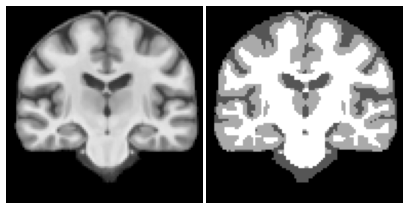
\includegraphics[scale=0.5]{atlas.png}
\end{center}
\end{frame}

\begin{frame}{Registration and Segmentation Support Each Other}

{\large Observation: \emph{\rcolor{registration} and \scolor{segmentation} support each other}.}

$$
\text{\scolor{seg} oracle} \quad + \quad \text{``anatomy loss''}\quad \rightarrow\quad \text{improved \rcolor{reg}}
$$
\begin{center}
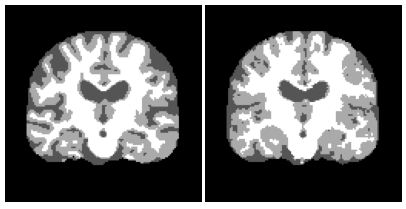
\includegraphics[scale=0.5]{anatomy_loss.png}
\end{center}
\end{frame}


\begin{frame}{Registration and Segmentation Support Each Other}

{\large Observation: \emph{\rcolor{registration} and \scolor{segmentation} support each other}.}

$$
\begin{array}{llll}
\text{\rcolor{reg} oracle} \quad &+ \quad \text{a labeled atlas}\quad &=\quad &\text{\scolor{seg} oracle}\\
\text{\scolor{seg} oracle} \quad &+ \quad \text{``anatomy loss''}\quad &\rightarrow\quad &\text{improved \rcolor{reg}}
\end{array}
$$

{\large Let's train registration and segmentation models \emph{jointly}:}

\vspace{1em}

Registration model loss:
$
\mathcal{L}_\text{sim}(I_m\circ \Phi, I_t)
+ \lambda_\text{reg} \mathcal{L}_\text{reg}(\Phi)
+ \lambda_\text{ana} \mathcal{L}_\text{ana}(S_m\circ \Phi, S_t)
$

Segmentation  model loss:
$
\lambda_\text{ana} {L}_\text{ana}
+ \lambda_\text{sp} \mathcal{L}_\text{sp}
$
\end{frame}


\begin{frame}{Overview Figure}
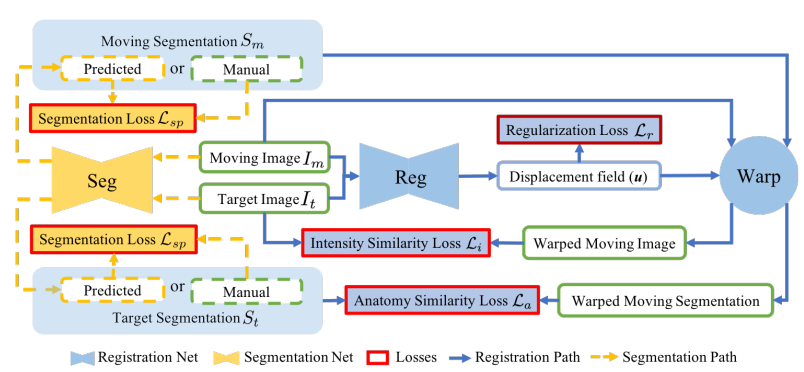
\includegraphics[scale=0.65]{figures/deepatlas-paper-fig.png}
\end{frame}

\begin{frame}{Registration Loss Flowchart}
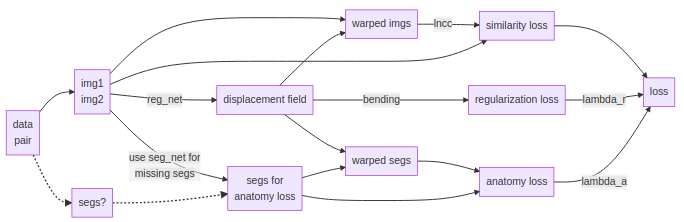
\includegraphics[scale=0.75]{figures/reg_loss_flowchart.png}
\end{frame}

\begin{frame}{Segmentation Loss Flowchart}
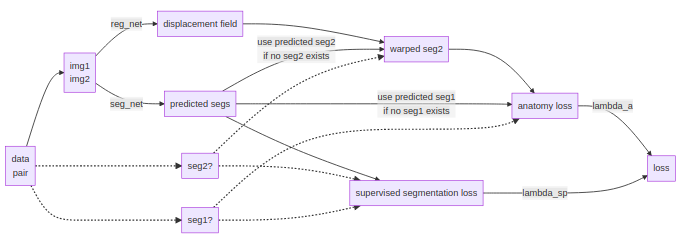
\includegraphics[scale=0.75]{figures/seg_loss_flowchart.png}
\end{frame}

\begin{frame}{Data Used in Tutorial Notebook}
OASIS-1, 416 subjects aged 18 to 96, T1-weighted MRI scans, tissue class segmentations

\begin{center}
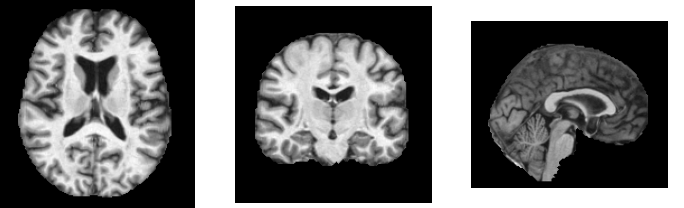
\includegraphics[scale=0.5]{oasis.png}
\end{center}

\vfill

\only<1>{\fullcite{oasis1}}
\only<2>{
Fine for demo, though not a natural DeepAtlas use case:
\begin{itemize}
\item tissue type segmentation from brain MRI is typically not manual
\item limitation of segmentation data is artificially imposed for the sake of demo
\end{itemize}
}
\end{frame}


\begin{frame}[fragile]{MONAI Networks}
\begin{minted}{python}
seg_net = monai.networks.nets.UNet(
	3,  # spatial dims
	1,  # input channels
	num_segmentation_classes,  # output channels
	(8, 16, 16, 32, 32, 64, 64),  # channel sequence
	(1, 2, 1, 2, 1, 2),  # convolutional strides
	dropout=0.2,
	norm='batch'
)
\end{minted}
\end{frame}

\begin{frame}[fragile]{MONAI Networks}
\begin{minted}{python}
reg_net = monai.networks.nets.UNet(
	3,  # spatial dims
	2,  # input channels (one for fixed image and one for moving image)
	3,  # output channels (to represent 3D displacement vector field)
	(16, 32, 32, 32, 32),  # channel sequence
	(1, 2, 2, 2),  # convolutional strides
	dropout=0.2,
	norm="batch"
)
\end{minted}
\end{frame}

\begin{frame}[fragile]{MONAI Warp}
	\begin{minted}{python}
warp = monai.networks.blocks.Warp(mode="bilinear", padding_mode="border")

ddf = reg_net(img_pair)
warped_moving_image = warp(moving_img, ddf)
	\end{minted}
\pause
\begin{center}
	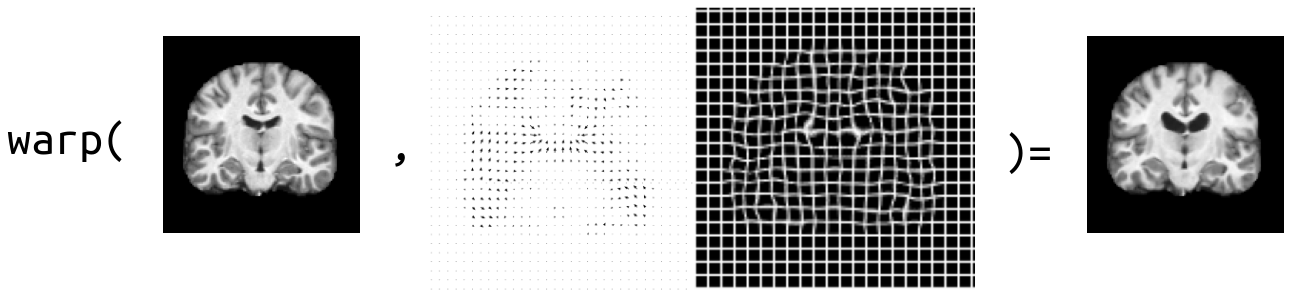
\includegraphics[scale=0.4]{ddf.png}
\end{center}
\end{frame}


\begin{frame}[fragile]{MONAI Losses}
\begin{minted}{python}
lncc_loss = monai.losses.LocalNormalizedCrossCorrelationLoss(
	spatial_dims=3,
	kernel_size=3,
	kernel_type='rectangular',
	reduction="mean"
)

bending_loss = monai.losses.BendingEnergyLoss(normalize = True)

loss_similarity = lncc_loss(warped_moving_image, target_image)
loss_regularization = bending_loss(ddf)
\end{minted}
\end{frame}



\begin{frame}{Notebook}
Find the notebook at
\url{https://github.com/Project-MONAI/tutorials/}

\vspace{2em}
	
Notebook is only a demo of the DeepAtlas approach.

For practically usable models:
\begin{itemize}
	\item add data augmentation (MONAI makes this super easy)
	\item package the model together with needed pre- and post-processing
\end{itemize}
\end{frame}


\begin{frame}{Where to Contribute}
\begin{itemize}
	\item Core
	\begin{itemize}
		\item \url{https://github.com/Project-MONAI/MONAI}
		\item useful transforms, network layers, network architectures, etc.
	\end{itemize}
	\item Tutorials
	\begin{itemize}
		\item \url{https://github.com/Project-MONAI/tutorials}
		\item show how to do something using MONAI
	\end{itemize}
	\item Research
	\begin{itemize}
		\item \url{https://github.com/Project-MONAI/research-contributions}
		\item published, peer-reviewed research
		\item good initial entry point for research code that has potential for going into core
	\end{itemize}
\end{itemize}
\end{frame}


\section{Slicer Integration}

\begin{frame}{LungAIR Clinical Platform}
\begin{itemize}
	\item Desktop application to help track progress of premature babies in NICU
	\item Goal is to incorporate AI models for BPD risk prediction
	\item Need:
	\begin{itemize}
		\item AI models that work with X-Rays and EHR data \only<2,3,4>{$\rightsquigarrow$ \textbf{MONAI}} 
		\item A desktop app that allows viewing and interacting with the results \only<3,4>{$\rightsquigarrow$ \textbf{3D Slicer}} 
	\end{itemize}
\end{itemize}
\only<1,2,3>{\vspace{11em}}
\only<4>{
\begin{center}

\includegraphics[scale=0.25]{logos/logo_monai}
\quad
\raisebox{4em}{\huge\ensuremath\varheartsuit}
\quad

\includegraphics[scale=0.5]{logos/logo_slicer}
\end{center}
}
\end{frame}

\begin{frame}{Using MONAI in Slicer}
Just pip install it
\begin{center}
	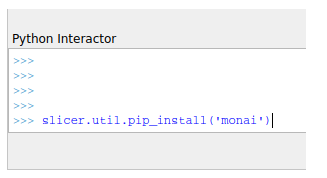
\includegraphics[scale=1]{figures/slicer_pip_install}
\end{center}
\end{frame}

\begin{frame}{Slicer + PyTorch}
But first install torch properly
\begin{center}
	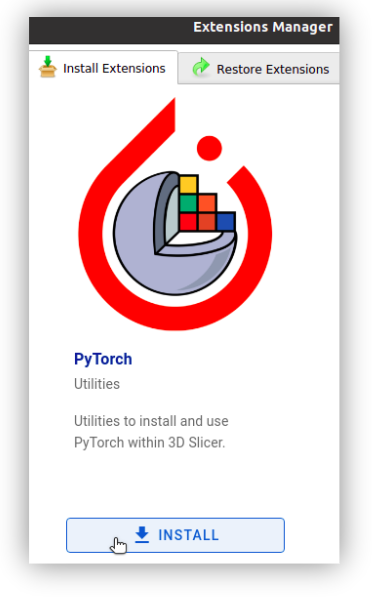
\includegraphics[scale=0.4]{figures/slicer-pytorch1}
	\hspace{3em}
	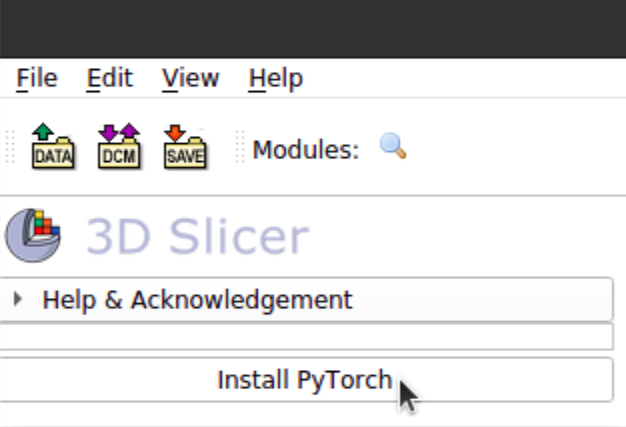
\includegraphics[scale=0.4]{figures/slicer-pytorch2}
\end{center}
\end{frame}

\begin{frame}{Inference in Slicer}
\begin{center}
	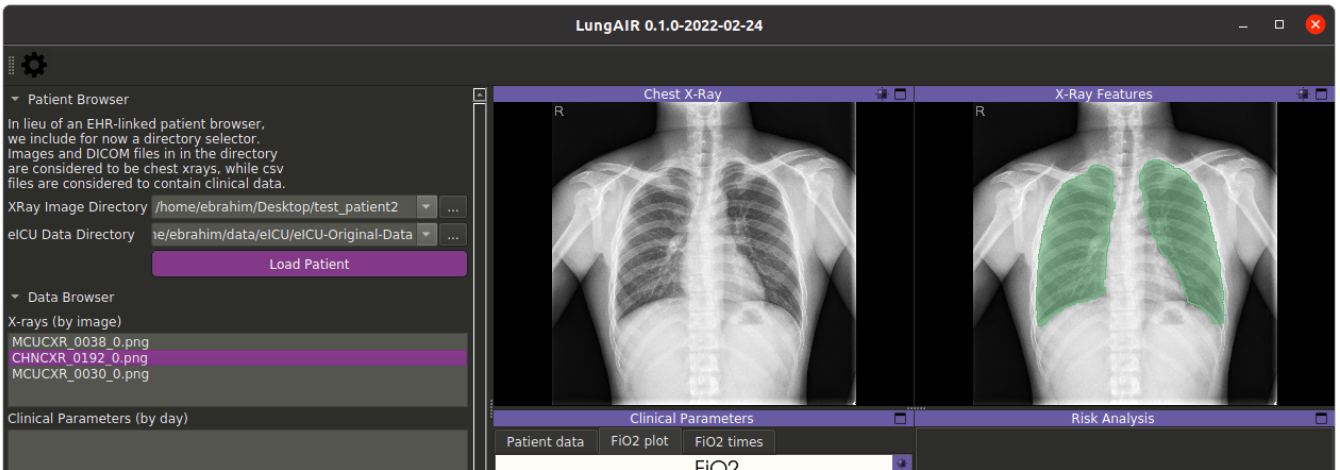
\includegraphics[scale=0.4]{figures/lungair}
\end{center}
\end{frame}

\begin{frame}[fragile]{Inference in Slicer}
\begin{minted}{python}
# Save model with some extra info
torch.save(
	{
		'model': seg_net.cpu(),
		'transform' : transform,
		'image_size': image_size,
	}, save_path)

# ... later in Slicer application
torch.load(...)
\end{minted}
Need the metadata to handle pre- and post-processing in Slicer.\\
MONAI Bundle was probably the way to go here...
\end{frame}




\section{Community}

\begin{frame}{Community}
\begin{itemize}
	\item Discussions
	\begin{itemize}
		\item \url{https://github.com/Project-MONAI/MONAI/discussions}
		\item everyone is super nice
	\end{itemize}
	\item Contributions
	\begin{itemize}
		\item read \url{https://github.com/Project-MONAI/MONAI/blob/dev/CONTRIBUTING.md}\\and get going!
		\item devs are very welcoming and helpful
	\end{itemize}
\end{itemize}
\end{frame}


\section{End}



\begin{frame}[standout]
\centering
{\huge Thanks!}\\
ebrahim.ebrahim@kitware.com\\
kitware@kitware.com\\
\vspace{1cm}
%{\Huge Questions?}\\
\end{frame}


\begin{frame}[allowframebreaks]{References}
\printbibliography
\end{frame}



\end{document}

